\documentclass[a4paper,12pt]{article}

\usepackage{amsmath, amssymb}
\usepackage{geometry}
\usepackage{enumitem}
\usepackage{fancyhdr}
\usepackage{xcolor}
\usepackage{sectsty}
\usepackage{multicol}
\usepackage{graphicx}
\usepackage{float}
\usepackage{array}
\usepackage{multirow}

\geometry{top=1in, bottom=1.5cm, left=1.5cm, right=1.5cm}

\pagestyle{empty}
\sectionfont{\color{blue}}

\begin{document}

% ================= HEADER =================
\thispagestyle{fancy}
\fancyhf{}

\fancyhead[L]{
    
\includegraphics[width=7cm]{logo.png}
}

\fancyhead[R]{
    Name: CHINMAYI V V \\
    Batch: COMETFWC041 \\
    Date: 20 FEB 2026
}

\renewcommand{\headrulewidth}{0pt}
\fancyfoot[C]{\thepage}

\vspace*{4cm}

% ================= TITLE =================
\begin{center}
{\LARGE \textbf{\textcolor{blue}{GATE 2010 EC - Question 12 Analysis}}}
\end{center}

% ================= QUESTION =================
\section*{Question 12}

For the output $F$ to be 1 in the logic circuit shown, the input combination should be:

\begin{center}
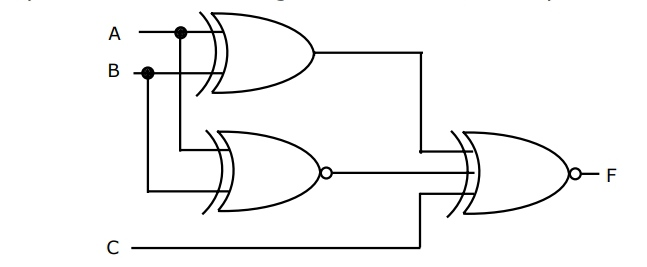
\includegraphics[width=10cm]{circuit.jpg}
\end{center}

\begin{multicols}{2}
\begin{enumerate}[label=\Alph*.]
\item A=1, B=1, C=0
\item A=1, B=0, C=0
\item A=0, B=1, C=0
\item A=0, B=0, C=1
\end{enumerate}
\end{multicols}

% ================= ANALYSIS =================
\section*{Question Analysis}

\begin{itemize}
\item Two input XOR gate: $X = A \oplus B$
\item Two input XNOR gate: $Y = A \odot B$
\item Three input XNOR gate: $F = X \odot Y \odot C$
\item Final expression:
\[
F = (A \oplus B) \odot (A \odot B) \odot C
\]
\end{itemize}

% ================= TRUTH TABLE =================
\section*{The Truth Table}

\begin{center}
\begin{tabular}{|c|c|c|c|}
\hline
A & B & C & F \\
\hline
0 & 0 & 0 & 0 \\
0 & 0 & 1 & 1 \\
0 & 1 & 0 & 0 \\
0 & 1 & 1 & 1 \\
1 & 0 & 0 & 0 \\
1 & 0 & 1 & 1 \\
1 & 1 & 0 & 0 \\
1 & 1 & 1 & 1 \\
\hline
\end{tabular}
\end{center}

% ================= HARDWARE =================
\section*{Hardware Implementation}

The circuit is implemented using Arduino UNO board.  
Inputs A, B, C are given through digital pins.  
Output F is verified using LED and seven segment display.

% == COMPONENTS ===
\section*{Required Components}

\begin{center}
\begin{tabular}{|c|l|}
\hline
S.No & Component \\ \hline
1 & Arduino Uno Board \\
2 & Breadboard \\
3 & Seven Segment Display \\
4 & 220$\Omega$ Resistors \\
5 & Jumper Wires \\
6 & USB Cable \\
\hline
\end{tabular}
\end{center}

%  PIN CONNECTIONS 
\section*{Pin Connections}

\begin{center}
\begin{tabular}{|c|c|}
\hline
Component & Arduino Pin \\ \hline
Input A & Digital 2 \\
Input B & Digital 3 \\
Input C & Digital 4 \\
LED Output F & Digital 12 \\
\hline
\end{tabular}
\end{center}

%  CODE UPLOADING 
\section*{Code Uploading Steps}

\begin{enumerate}
\item Create PlatformIO project
\item Write code in main.cpp
\item Run command: pio run
\item Copy generated .hex file
\item Connect Arduino using OTG
\item Upload using "Upload Precompiled"
\item Verify output
\end{enumerate}

% ==== OUTPUT IMAGE ======
\section*{Experimental Output}

\begin{center}
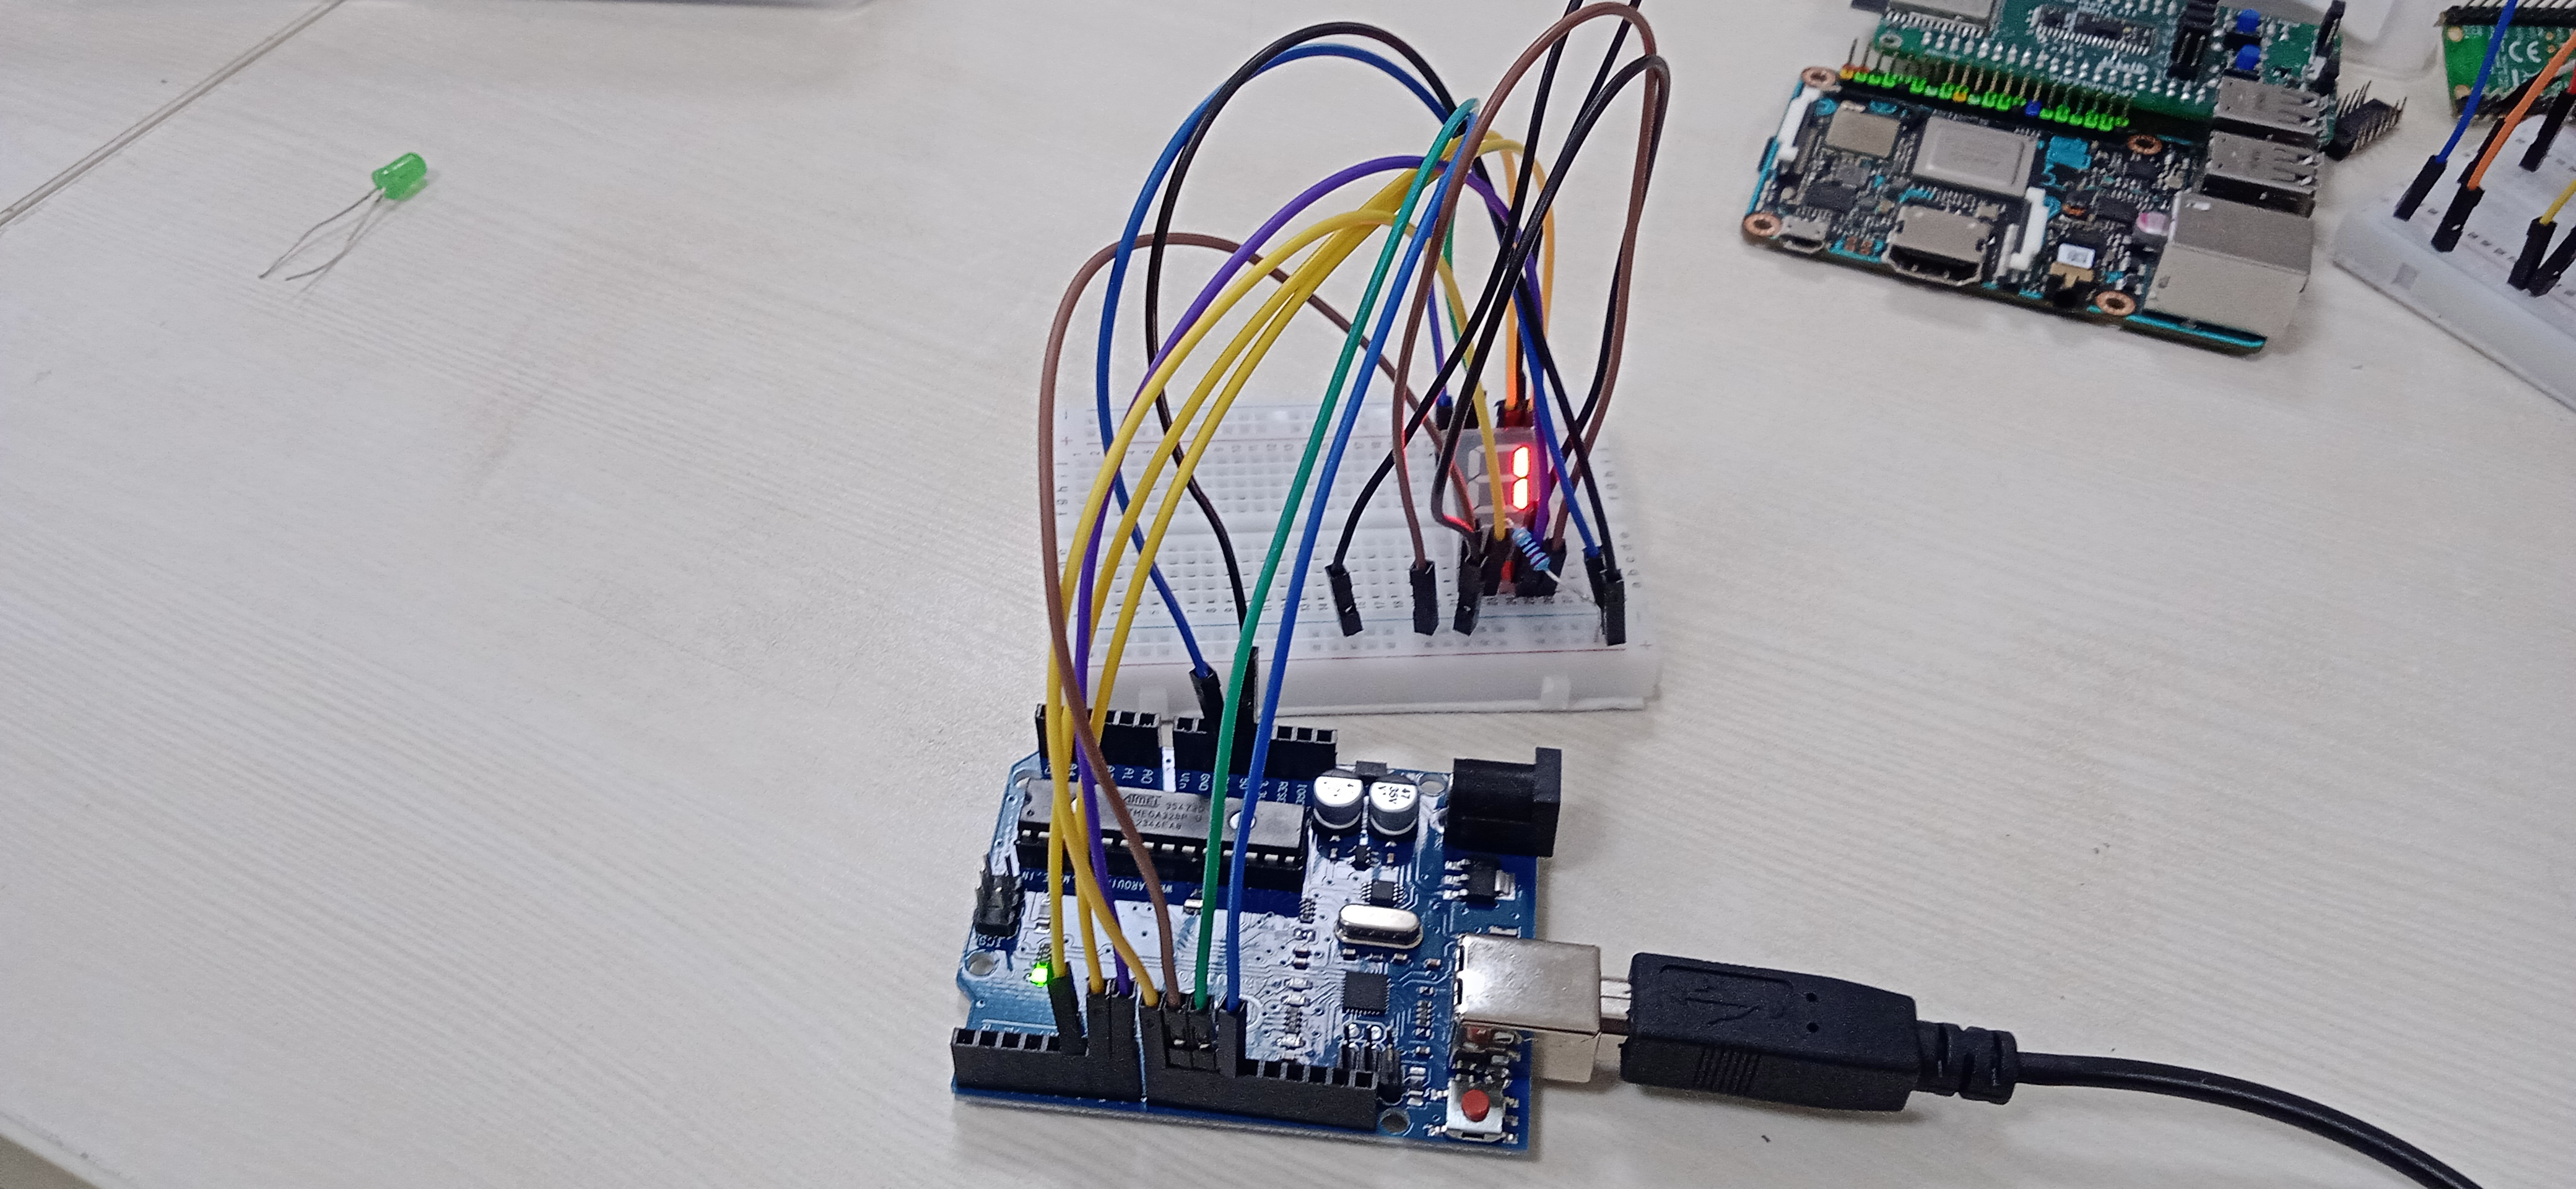
\includegraphics[width=8cm]{output.jpg}
\end{center}

%  CONCLUSION 
\section*{Conclusion}

From the truth table, $F=1$ whenever $C=1$.  
Hence the correct option is:

\[
\boxed{\text{Option (D)}}
\]

The hardware implementation confirms the theoretical logic.

\end{document}
